\documentclass[10pt]{article}
\usepackage[utf8]{inputenc}

\usepackage{graphicx} % Required for inserting images
\usepackage{multicol}
\usepackage{wrapfig}
\usepackage{float}

\usepackage{hyperref}
\usepackage{svg}
\usepackage{subfig}
\usepackage{siunitx}

\usepackage[%
    a4paper,
    top=1.2cm,
    bottom=1.6cm,
    left=1.8cm,
    right=1.8cm,
    marginparwidth=1.75cm
]{geometry}

\title{RS: Third Homework}
\author{
    Mark Loboda in Simon Goričar
}
\date{15. 5. 2025}

\begin{document}
\maketitle

\section{Benchmarks}

\subsection{Task 1: Multilayer Perceptron (MLP) and Digit Recognition}



\subsection{Task 2: K-means clustering and image processing}
In this task, we implemented and benchmarked a vectorized version of the K-means clustering algorithm for grayscale image quantization. The core functions \texttt{assign\_points\_to\_clusters} and \texttt{update\_centroids} were initially written in scalar C. We used the AVX intrinsics to improve performance. The effectiveness of the optimization was evaluated using the \texttt{rdtsc()} function to measure the CPU cycles required to compute the result. We then computed the resulting speedup ratios across multiple configurations of the algorithm.

The configurations included using 4, 8, and 16 clusters with both single- and double- precision data.

\begin{figure*}[htbp]
    \centering
    \subfloat[]{%
        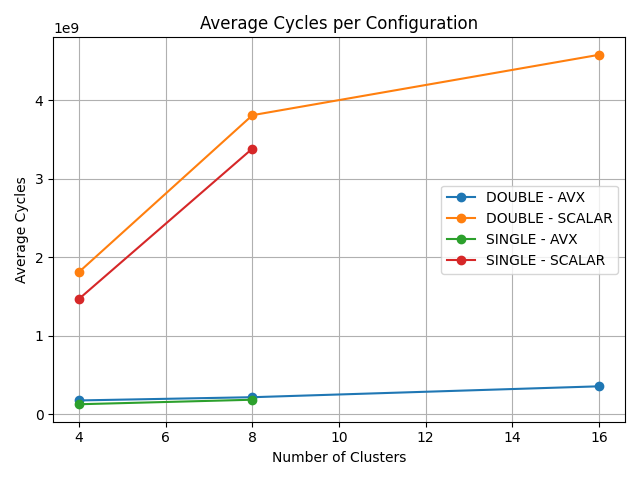
\includegraphics[width=0.45\linewidth]{images/task2/avg_cycles_per_config.png}
        \label{fig:task2:cpi}
    }\hfill
    \subfloat[]{%
        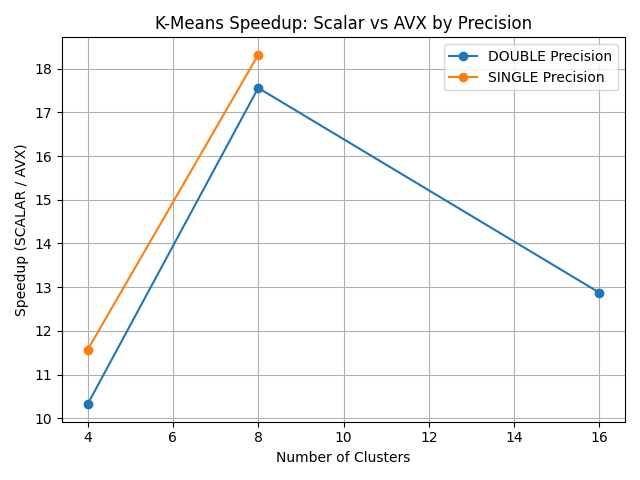
\includegraphics[width=0.45\linewidth]{images/task2/speedup_vs_clusters.png}
        \label{fig:task2:cache_invalidations}
    }\\
    \caption{Results of the K-means algorithm benchmarking. Left figure shows the average number of cycles per algorithm. The right figure shows speedups for the same algorithms, where $speedup = CYCLES_{scalar} / CYCLES_{AVX}$}
    \label{fig:task2:speedup}
\end{figure*}

The AVX-vectorized implementation of the K-means significantly outperformed the scalar version across all configurations. The largest speedups were seen in configurations with 8 clusters.

When comparing single- and double- precision implementations, the results show a better speedup with single precision. This is expected because twice as many floats can be processed at once.

The results in the figure~\ref{fig:task2:speedup} show a substantial gain on all configurations of the vectorized compared to the scalar implementation. A change to single precision compared to double didn't increase the performance much, as the algorithm for 4 clusters had to use the 128-bit registers and couldn't do more work in parallel. This could, however be further optimized to do more work in parallel. The vectorization had the biggest impact when running the algorithm on 8 clusters but fell off, when running with 16. This is because the scalar implementation scaled much better from 8 to 16 clusters compared to 4 to 8 clusters, while the vectorized algorithm scaled linearly through all configurations.

To conclude, the AVX vectorization of K-means greatly enhanced performance across all cluster counts. It scaled much better with the number of clusters. The speedup somewhat reduced when increasing the number of clusters from 8 to 16, because the scalar implementation scaled much better on this step, while the vectorized version scaled linearly.

\end{document}
